% Chapter Template

\chapter{Control} % Main chapter title

\label{Chapter 3} % Change X to a consecutive number; for referencing this chapter elsewhere, use \ref{ChapterX}

\lhead{Chapter 3. \emph{Control}} % Change X to a consecutive number; this is for the header on each page - perhaps a shortened title

%
Once the simulation is fully implemented, the goal is to use it as a testbench for different ways of controlling the structure. The second part of the project will be fully consecrated on this part. A few tools have been implemented to test some of the algorithms that are used in such problems. 

\section{PID Control of the joints}

One of the problem to control accurately a joint is to adapt the command so that it can adapt to difficult situation. For instance, it is easier to walk in a swimmingpool than on the ground and this is why people recovering after an injury do aquatic training. For a joint, it can be easy to do a movement in the air, but the same movement is more difficult when touching the ground. One way to avoid this problem is to implement PID (Proportional Integral Derivative) controller. This kind of controller is used in a lot of different situation in the world of automation to control degrees of freedom. In or case, servomotors often integrate such loops to account for these changes of use. In the simulation, at each step, the command of each degree of freedom of the structure is calculated using such a PID controller. 

\begin{figure}[htbp]
    \centering
    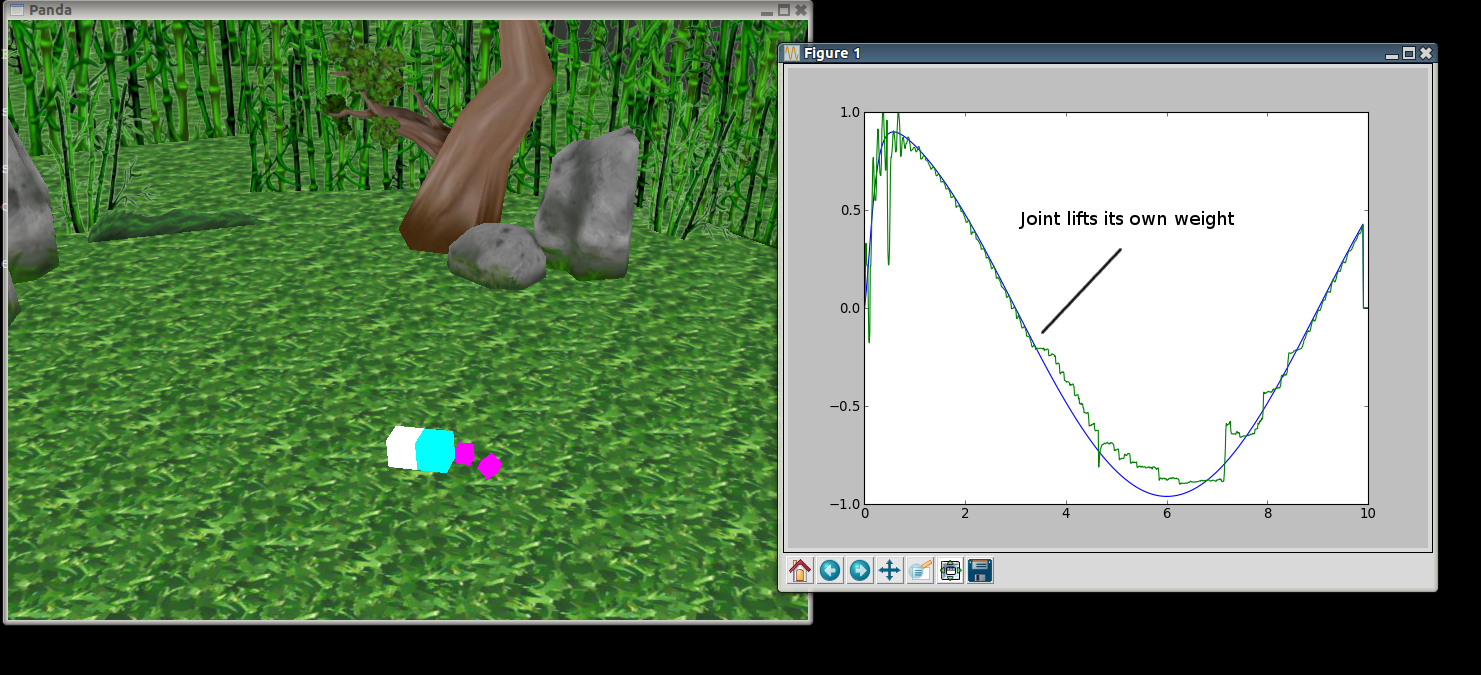
\includegraphics[scale=0.3]{Figures/servomotor.png}
    \rule{35em}{0.5pt}
    \caption[Answer of a joint to a sinusoid command]{Answer of the joint to a sinusoid command with PID Control}
    \label{fig:Snake}
\end{figure}

One of the problem with the control of the joints is the unstability. On the simulation, as the angles have periodic values, if the joint has a high angle velocity, then between two steps, it can jump accross the boundary and start turning faster and faster as the PID controller will not be able to work as well as if the degree of freedom were a linear parpameter. The problem with this situation is that it can actually be seen as a good result for the learning algorithm, simply because the fitness function is the velocity of the creature. There are several things to prevent from this situation :

\begin{itemize}
    \item reduce the time between two steps of computation for the physics engine and the PID
    \item reduce the maximum torque available per joint
    \item punish the creature if the joints are moving to slow
    \item change the fitness function to maximize parameter under a certain energy level
\end{itemize}
        

Another issue is more a biological concern. The main goal of this project is to find solutions that are biologically inspired instead of using a classical automation approach (eventhough we can compare the elasticity of or muscles as such controllers\ldots). Therefore though the use of PID is necessary in many robotics applications, we will try to avoid using the in the second part of the project. 

\section{Central Pattern Generator}

Central Pattern Generators (CPGs) are neural networks, that can generate oscillation for the control of the muscles of or body. They are the consequence and the cause of the paradigm of periodic movement in the locomation of animals. Different models have been implemented to represent CPGs. We can represent them as a graph of coupled oscillator, where each node influence the behavior of its neighbours. For a first implementation I choose to test the model of CPG followed at EPFL (\cite{sproewitz}). 

The CPG Neural Network in that case, is a graph that follow the physical architecture of the robot, settting one node for each joint (hinge or vertebra) on the structure. The dynamic of the CPG is determined by a coupling weight matrix $w_{ij}$, a phase bias matrix between nodes $\varphi_{ij}$, the frequency of the different oscillator $\omega_i$ and the desired amplitude and offset of the oscillation. We can compute the angle using the following system of equation and an integration method (I used the Runge-Kutta method in this project)

\begin{equation*}
    \dot{\phi_i} = \omega_i + \sum{w_{ij} * r_j * sin(\phi_i - \phi_j - \varphi_{ij})} \tag{1}
\end{equation*}
\begin{equation*}
        \theta_i = x_i + r_i * cos(\phi_i)  \tag{2}
\end{equation*}
This two equation gives the angle of the oscillator ($\theta_i$) depending on the state variable of a node: $x_i$, $r_i$, $\phi_i$, that can be described respectively as the offset, the amplitude and the phase of the oscillator.

\begin{equation*}
    \acute{r_i} = ar(\frac ar (R_i - r_i) - \dot{r_i}) \tag{3}
\end{equation*}
\begin{equation*}
    \acute{x_i} = ax(\frac ax (X_i - x_i) - \dot{x_i}) \tag{4}
\end{equation*}

Equations (3) and (4) describe the dynamic of the amplitude and offset (a second order dynamic that converge to the desired values). This trick is to ensure continuity in the oscillations, even if some of the parameters of the oscillator change. $a_r$ and $a_x$ are gains to control the dynamic ($a_r = a_x = 20 rad/s$  \cite{sproewitz}). 


A modification of this model is possible to plug the measured value of the degrees of freedom. Instead of using the second order control loop on $\theta_i$ which is achieved with the PID, we can set this control on the phase. Thatway, if the joint has troubles achieving his movement, for instance when hitting the ground, the phase will be modified and the perturbation will have an impact on othe joints through equation (1).

Oneway to do so is to add a term in the equation (1), with $\dot{\theta_{reali}}$ the mesured angle velocity of the joint. 
\begin{equation*}
    \dot{\phi_i} = \omega_i + \sum{w_{ij} * r_j * sin(\phi_i - \phi_j - \varphi_{ij}) + a_{\phi} * \frac {\dot{\theta_{reali}} - \dot{\theta_i}} {r_i * sin (\phi_i)}} \tag{1}
\end{equation*}

If we derive (2) we get: 
\begin{equation*}
    \dot{\theta_i} = \dot{x_i} + \dot{r_i} * cos(\phi_i) + r_i * sin(\phi_i) * \dot{\phi_i} \tag{2'}
\end{equation*}

By making the assumption that the dynamic of the amplitude and the offset is slow compared to the phase, we get
\begin{equation*}
    \dot{\theta_i} = r_i * sin(\phi_i) * \dot{\phi_i} \tag{2''}
\end{equation*}
Thatway, if we consider small variation of the phase, we can deduce an error term on $\dot{\phi_i}$ from the error on $\dot{\theta_i}$ given by $\frac {\dot{\theta_{reali}} - \dot{\theta_i}} {r_i * sin (\phi_i)}$ that we can control with a gain ($a_{\phi}$).
For example if the movement of a joint is made difficult because of the ground, then the mesured velocity of this joint will be smaller that expected. The consequence will be to accelerate the movement for this joint (the derivative of the phase will be bigger), but also for the other joints that are linked to this one. We can interprete this as neural communication in our body within the central pattern generator, but also as the elasticity between joints. For instance if achieving a movement is too difficult for a joint, using elasticity, it is possible to get help from joints that are near. 



